\documentclass{beamer}
\usepackage[utf8]{inputenc}

\usetheme{Madrid}
\usecolortheme{default}
\useinnertheme{circles}

\definecolor{Logo1}{rgb}{0.208, 0.2865, 0.373}
\definecolor{Logo2}{rgb}{0.000, 0.674, 0.863}

\setbeamercolor*{palette primary}{bg=Logo1, fg=white}
\setbeamercolor*{palette secondary}{bg=Logo2, fg=white}
\setbeamercolor*{palette tertiary}{bg=white, fg=Logo1}
\setbeamercolor*{palette quaternary}{bg=Logo1,fg=white}
\setbeamercolor{structure}{fg=Logo1} % itemize, enumerate, etc
\setbeamercolor{section in toc}{fg=Logo1} % TOC sections

%------------------------------------------------------------
%This block of code defines the information to appear in the
%Title page
\title[] %optional
{Amazon Food Review}

\subtitle{LDA Topic Modeling with NLP\\
\& Sentiment Analysis
}

\author[] % (optional)
{Muhammed Berk Önder}

\institute[] % (optional)
{
  Istanbul Data Science Academy
}

\date[] % (optional)
{March 2022}

\setbeamertemplate{background}
{
    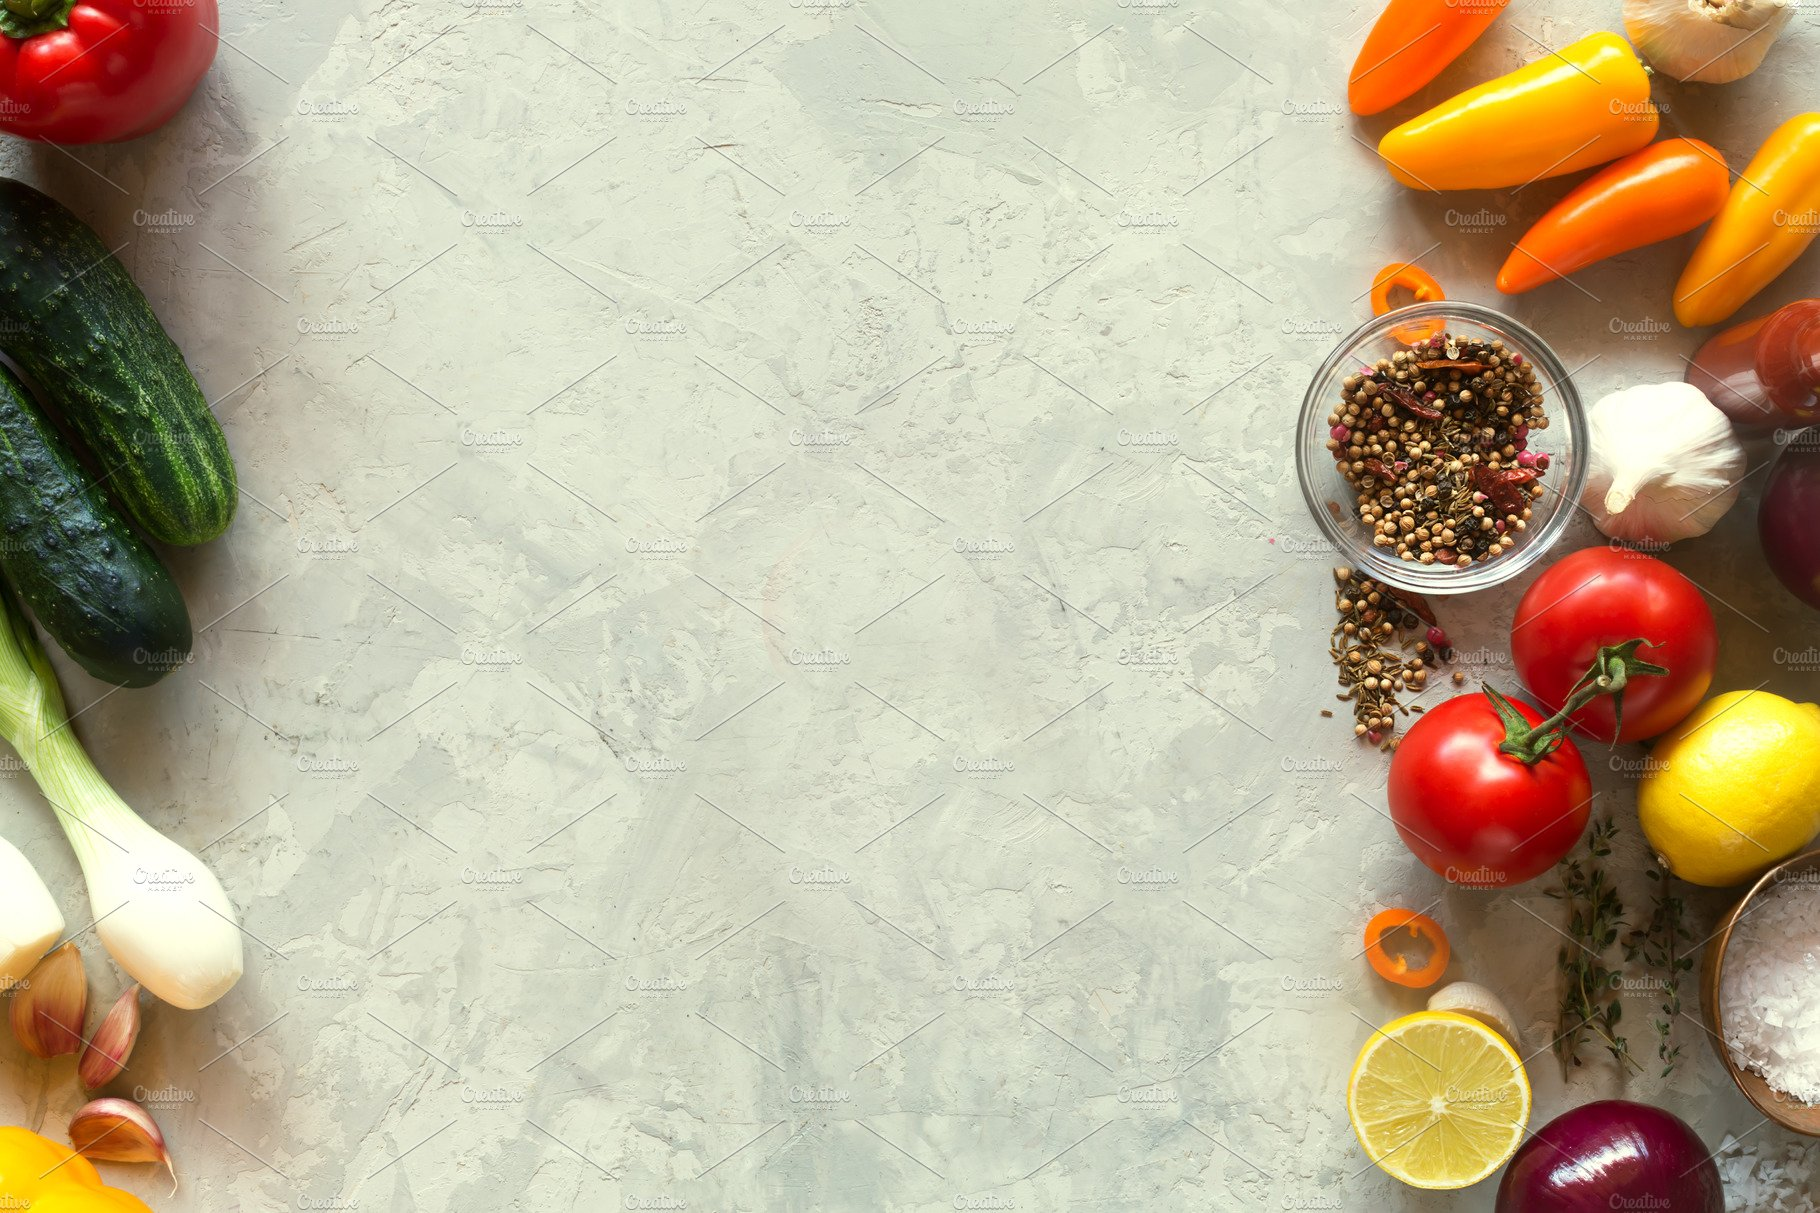
\includegraphics[width=\paperwidth, height=\paperheight]{img/MyBackground.jpg}
}

% \logo{\includegraphics[height=.5cm]{logo-footer.png}}

%End of title page configuration block
%------------------------------------------------------------



%------------------------------------------------------------
%The next block of commands puts the table of contents at the 
%beginning of each section and highlights the current section:

\AtBeginSection[]
{
  \begin{frame}
    \frametitle{Table of Contents}
    \tableofcontents[currentsection]
  \end{frame}
}
%------------------------------------------------------------


\begin{document}

%The next statement creates the title page.
\frame{\titlepage}

\setbeamertemplate{background}
{
    
\includegraphics[width=\paperwidth, height=\paperheight]{img/white.jpg}
}

%---------------------------------------------------------
%This block of code is for the table of contents after
%the title page
\begin{frame}
\frametitle{Table of Contents}
\tableofcontents
\end{frame}
%---------------------------------------------------------

\section{Methodology}

%---------------------------------------------------------
%Changing visivility of the text
\begin{frame}
\frametitle{Methodology}
\begin{itemize}
    \item Collect data from MongoDB with PyMongo
    \item Clean and Tokenize Data
    \item CV and TF-IDF
    \item Latent Dirichlet Allocation
    \item Model Results
\end{itemize}
\end{frame}

%---------------------------------------------------------

\section{Database}

%---------------------------------------------------------
%Example of the \pause command
\begin{frame}
    \begin{figure}
        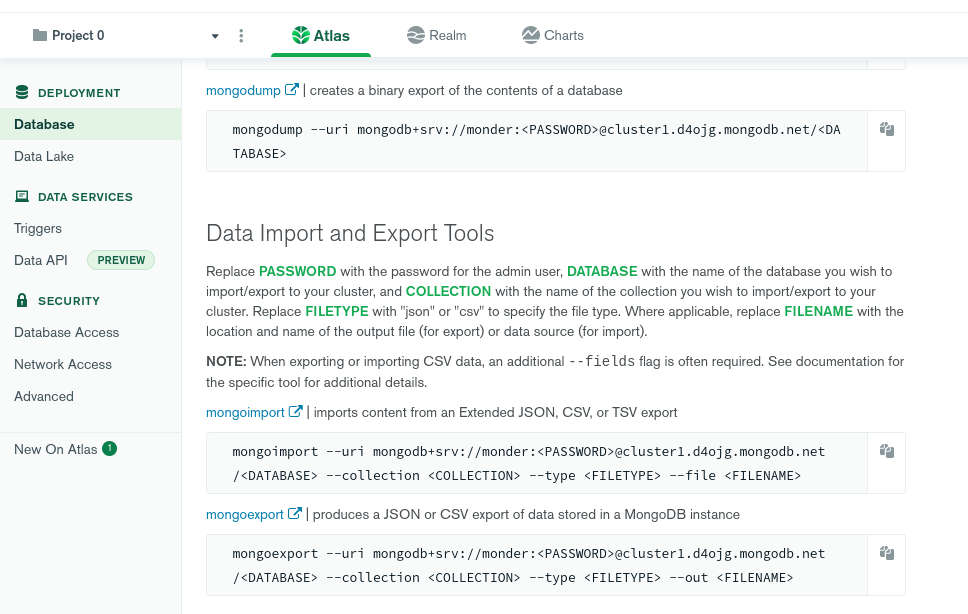
\includegraphics[width=\textwidth]{../figures/mongo_import.png}
    \end{figure}
\end{frame}
%---------------------------------------------------------

%---------------------------------------------------------
%Example of the \pause command
\begin{frame}
    \begin{figure}
        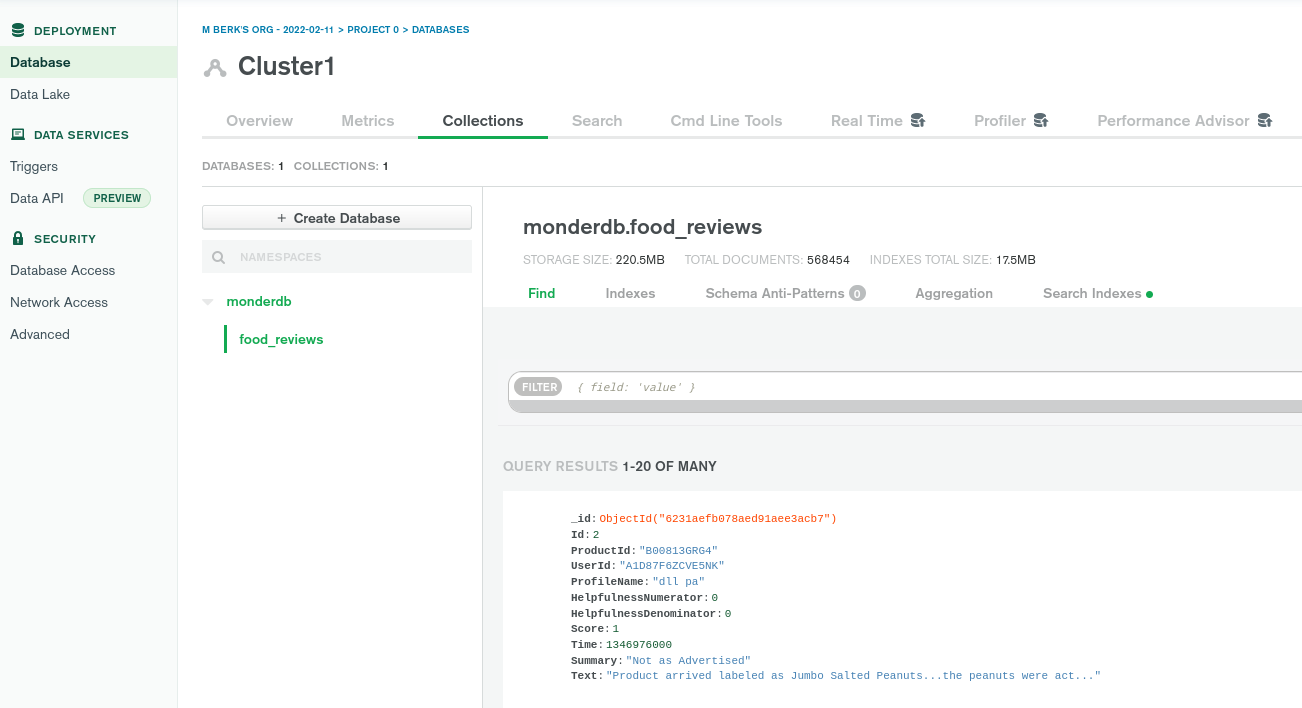
\includegraphics[width=\textwidth]{../figures/mongo_cluster.png}
    \end{figure}
\end{frame}
%---------------------------------------------------------

%---------------------------------------------------------
%Example of the \pause command
\begin{frame}
    \begin{figure}
        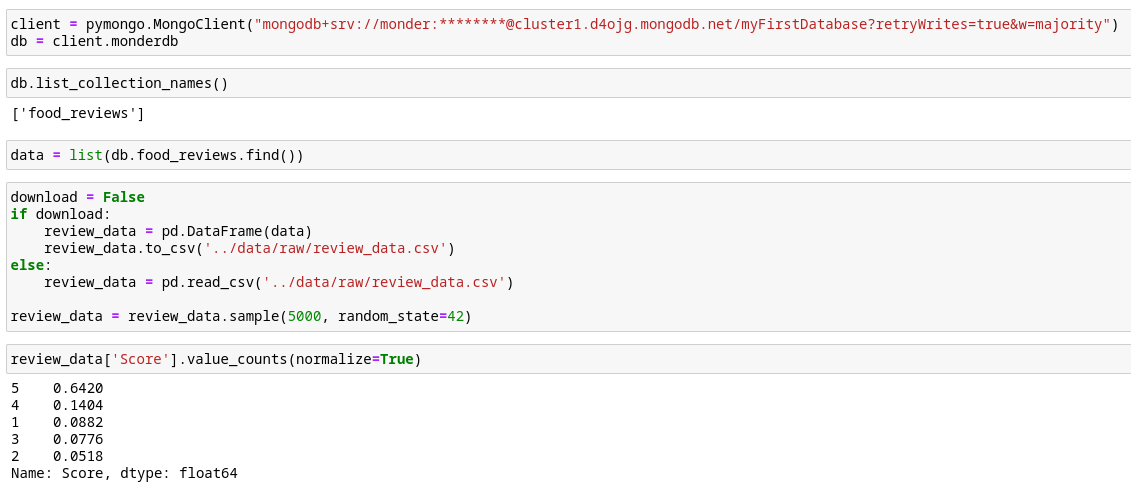
\includegraphics[width=\textwidth]{../figures/mongo_to_csv.png}
    \end{figure}
\end{frame}
%---------------------------------------------------------

\section{Preprocess}

%---------------------------------------------------------
%Example of the \pause command
\begin{frame}
    \begin{figure}
        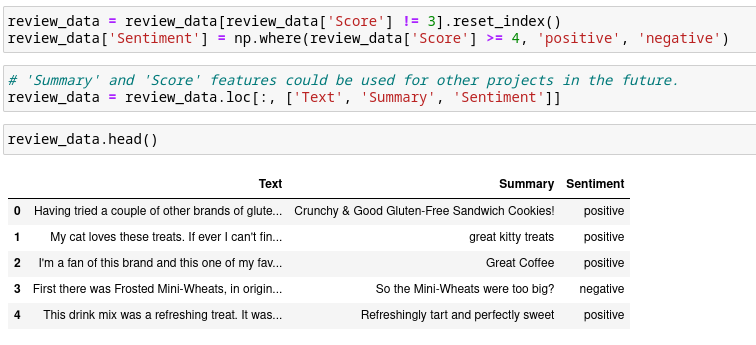
\includegraphics[width=\textwidth]{../figures/pre_sentiment.png}
    \end{figure}
\end{frame}
%---------------------------------------------------------

%---------------------------------------------------------
%Example of the \pause command
\begin{frame}
    \begin{figure}
        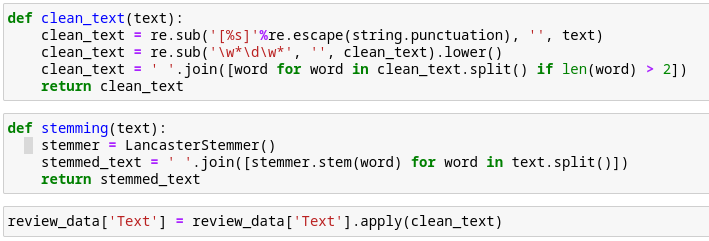
\includegraphics[width=\textwidth]{../figures/pre_clean.png}
    \end{figure}
\end{frame}
%---------------------------------------------------------

%---------------------------------------------------------
%Example of the \pause command
\begin{frame}
    \begin{figure}
        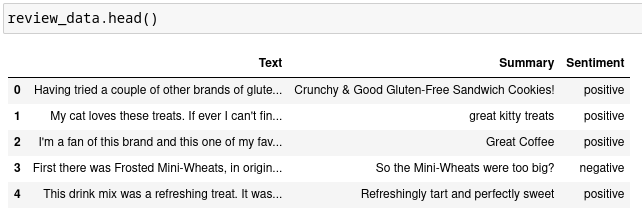
\includegraphics[width=\textwidth]{../figures/pre_before.png}
    \end{figure}
    \begin{figure}
        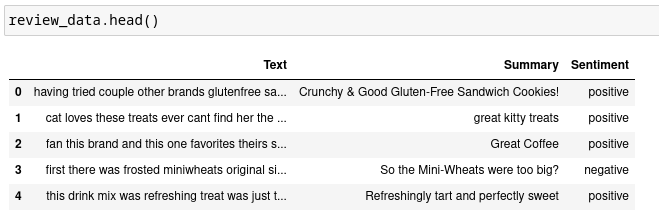
\includegraphics[width=\textwidth]{../figures/pre_after.png}
    \end{figure}
\end{frame}
%---------------------------------------------------------

\section{Sentiment}

%---------------------------------------------------------
%Example of the \pause command
\begin{frame}
    \begin{figure}
        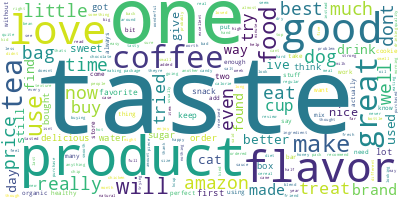
\includegraphics[width=.6\textwidth]{../figures/sent_wordcloud.png}
    \end{figure}
\end{frame}
%---------------------------------------------------------

%---------------------------------------------------------
%Example of the \pause command
\begin{frame}
    \begin{figure}
        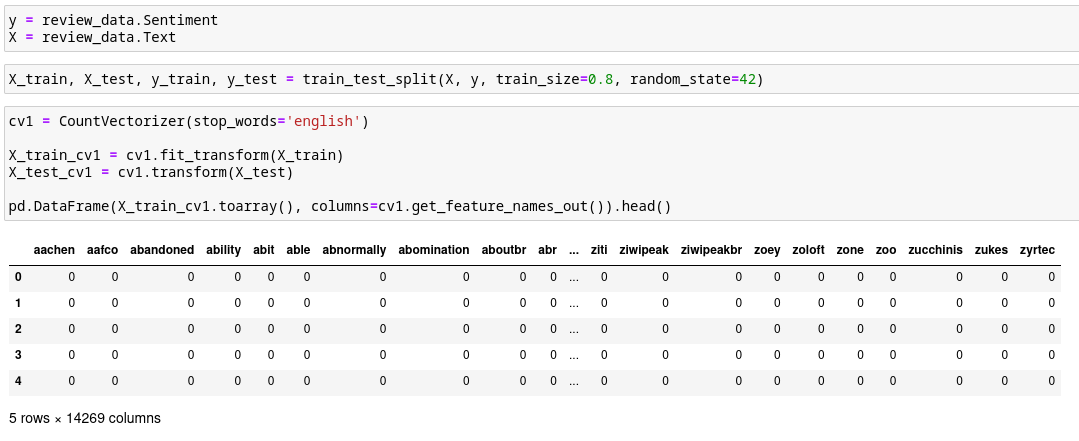
\includegraphics[width=\textwidth]{../figures/sent_cv1.png}
    \end{figure}
\end{frame}
%---------------------------------------------------------

%---------------------------------------------------------
%Example of the \pause command
\begin{frame}
    \begin{figure}
        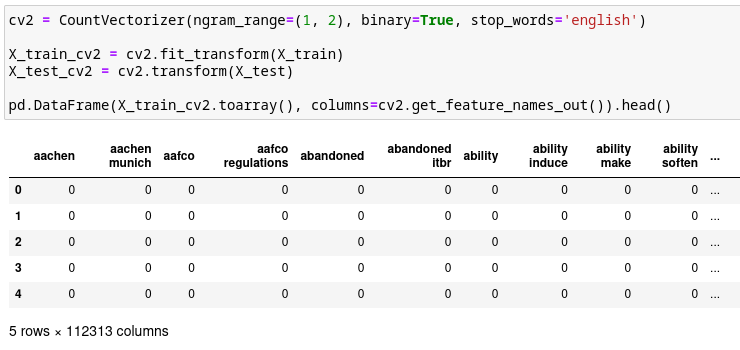
\includegraphics[width=\textwidth]{../figures/sent_cv2.png}
    \end{figure}
\end{frame}
%---------------------------------------------------------

\section{Topic Modeling}

%---------------------------------------------------------
%Example of the \pause command
\begin{frame}
    \begin{figure}
        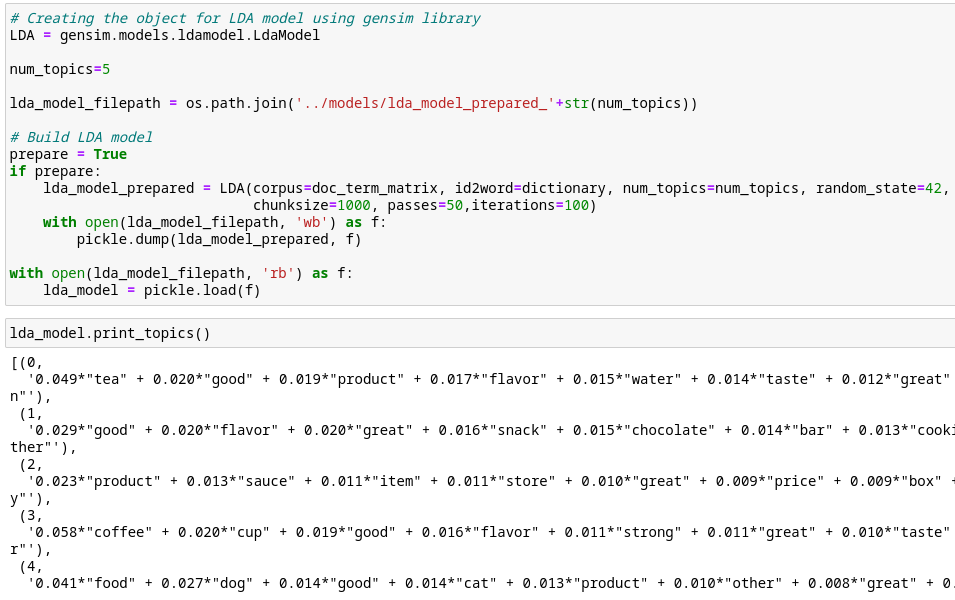
\includegraphics[width=\textwidth]{../figures/topic_lda.png}
    \end{figure}
\end{frame}
%---------------------------------------------------------

%---------------------------------------------------------
%Example of the \pause command
\begin{frame}
    \begin{figure}
        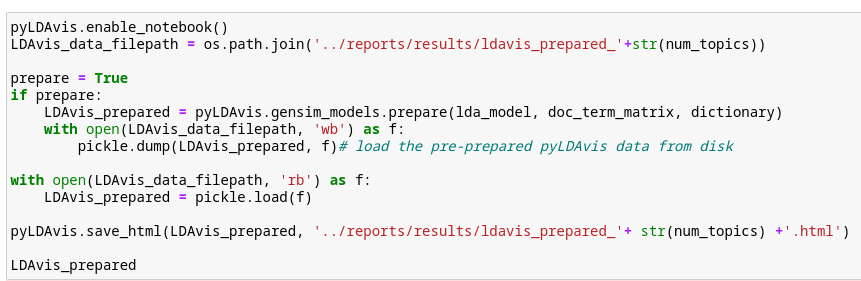
\includegraphics[width=\textwidth]{../figures/topic_gensim.png}
    \end{figure}
\end{frame}
%---------------------------------------------------------

\section{Results}

%---------------------------------------------------------
%Example of the \pause command
\begin{frame}
    \begin{figure}
        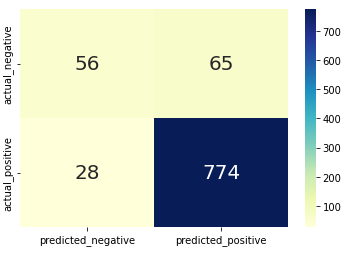
\includegraphics[width=.5\textwidth]{../figures/result_cm1.png}
    \end{figure}
    \begin{figure}
        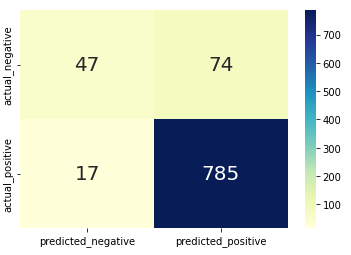
\includegraphics[width=.5\textwidth]{../figures/result_cm2.png}
    \end{figure}
\end{frame}
%---------------------------------------------------------

%---------------------------------------------------------
%Example of the \pause command
\begin{frame}
    \begin{figure}
        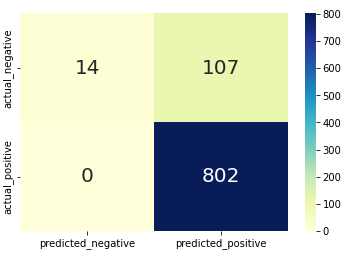
\includegraphics[width=.5\textwidth]{../figures/result_cm5.png}
    \end{figure}
    \begin{figure}
        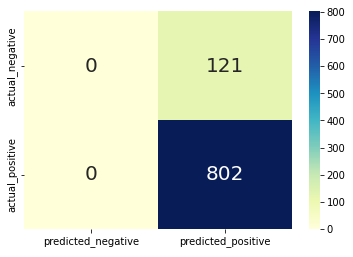
\includegraphics[width=.5\textwidth]{../figures/result_cm6.png}
    \end{figure}
\end{frame}
%---------------------------------------------------------

%---------------------------------------------------------
%Example of the \pause command
\begin{frame}
    \begin{figure}
        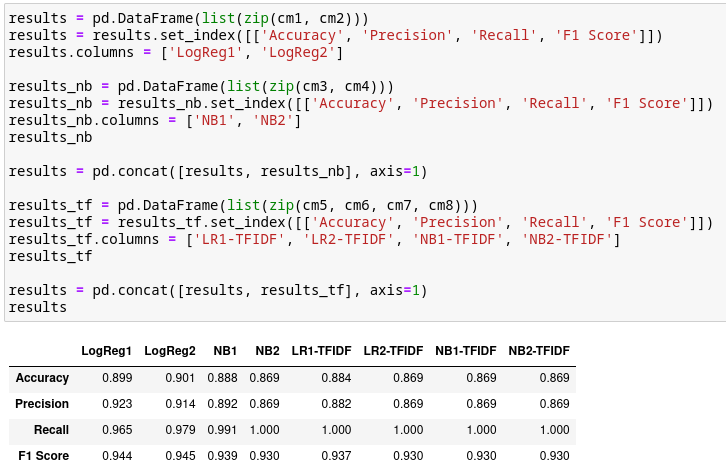
\includegraphics[width=\textwidth]{../figures/result_all.png}
    \end{figure}
\end{frame}
%---------------------------------------------------------

%---------------------------------------------------------
%Example of the \pause command
\begin{frame}
    \begin{figure}
        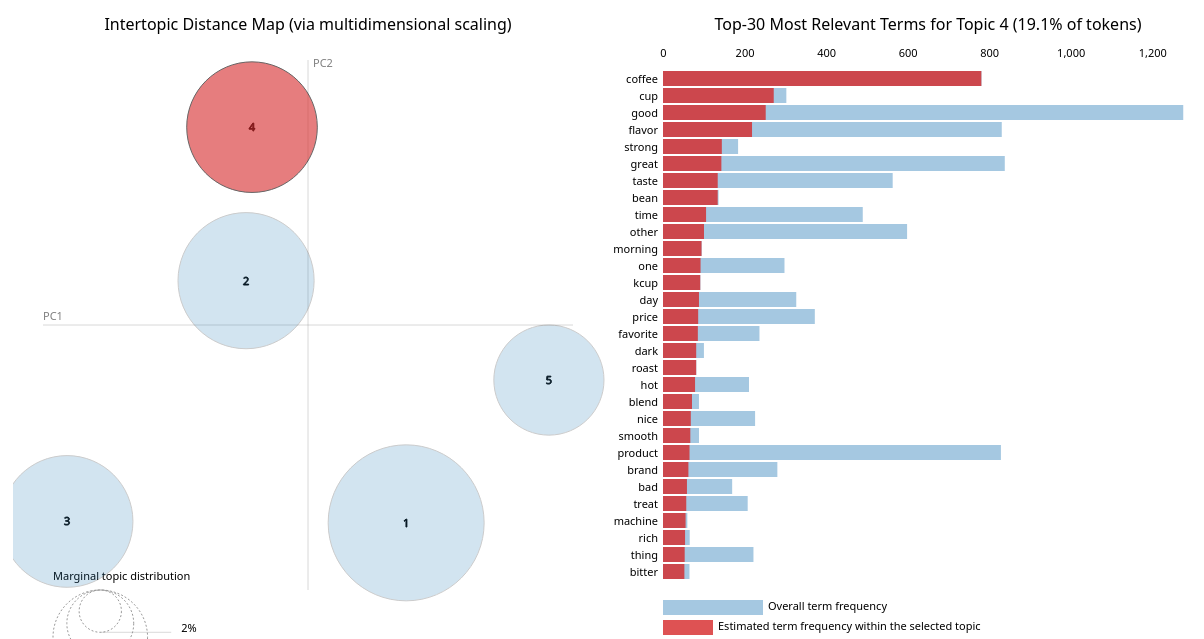
\includegraphics[width=\textwidth]{../figures/result_coffe.png}
    \end{figure}
\end{frame}
%---------------------------------------------------------

%---------------------------------------------------------
%Example of the \pause command
\begin{frame}
    \begin{figure}
        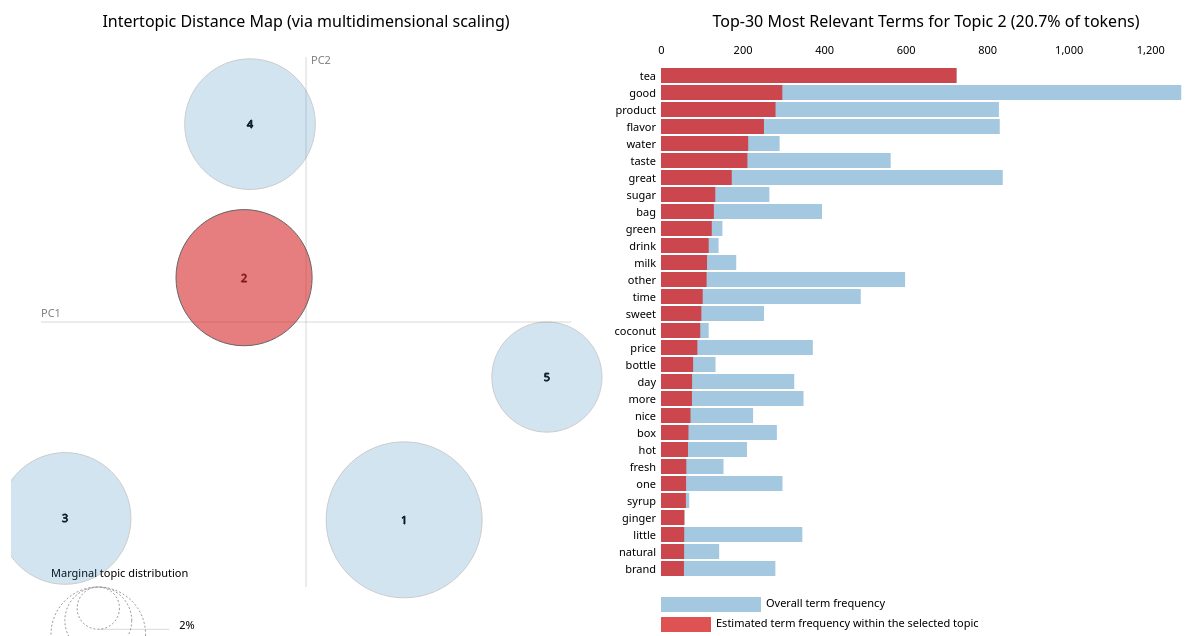
\includegraphics[width=\textwidth]{../figures/result_tea.png}
    \end{figure}
\end{frame}
%---------------------------------------------------------

%---------------------------------------------------------
%Example of the \pause command
\begin{frame}
    \begin{figure}
        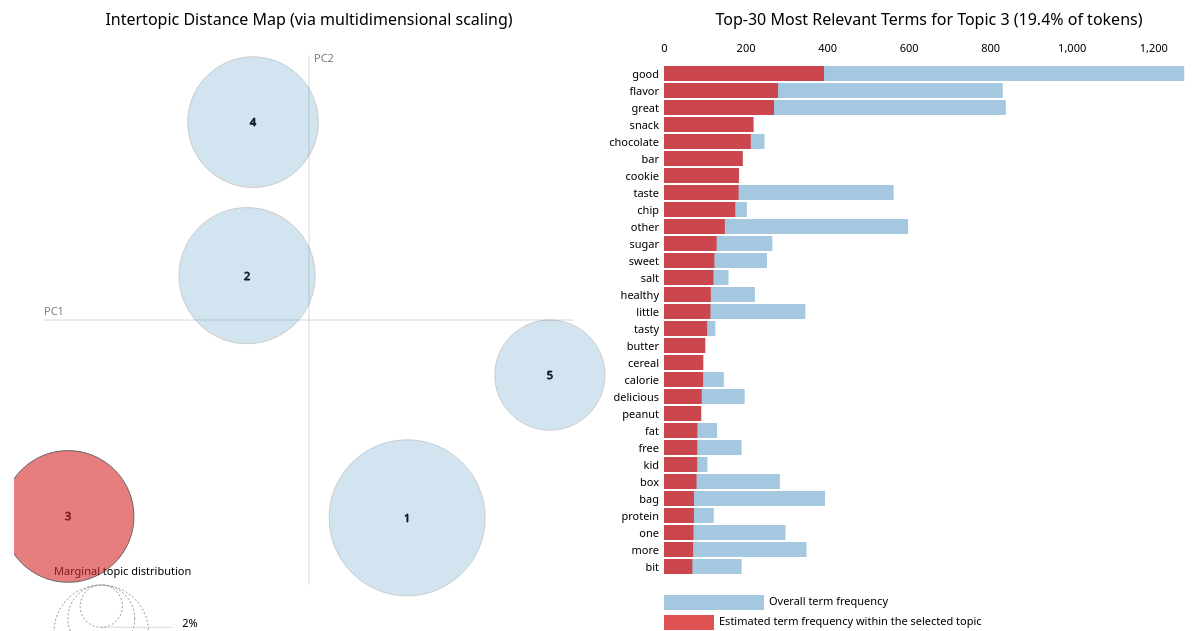
\includegraphics[width=\textwidth]{../figures/result_snack.png}
    \end{figure}
\end{frame}
%---------------------------------------------------------

%---------------------------------------------------------
%Example of the \pause command
\begin{frame}
    \begin{figure}
        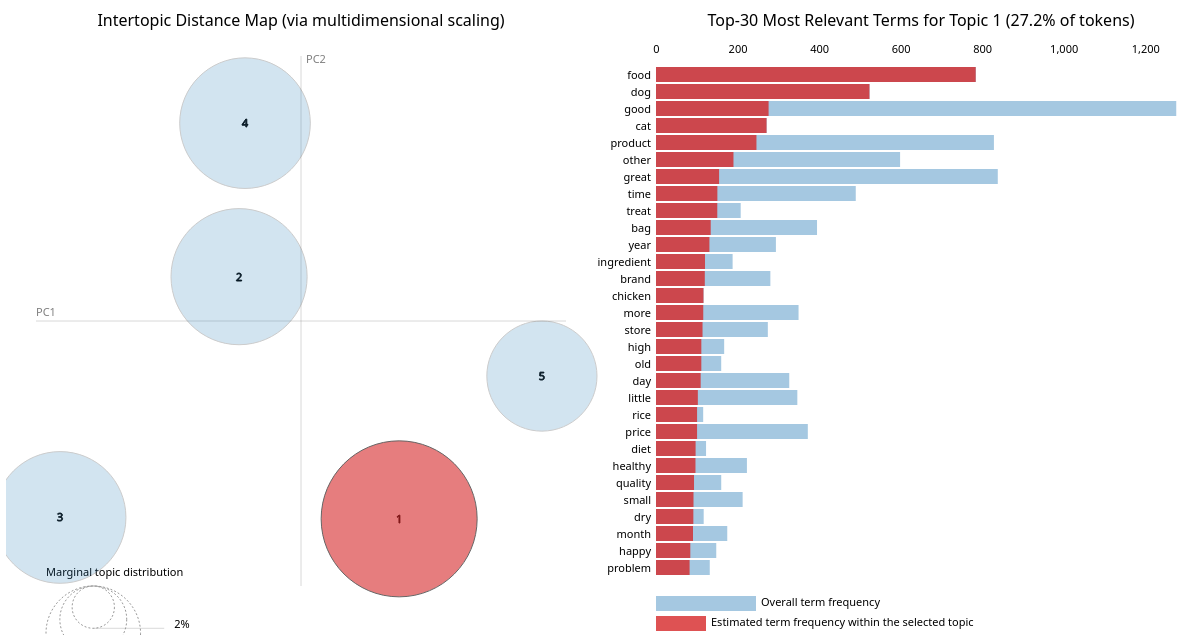
\includegraphics[width=\textwidth]{../figures/result_pet.png}
    \end{figure}
\end{frame}
%---------------------------------------------------------

\section{Future Work}

\begin{frame}
    \frametitle{Future Work}
    \centering
    \begin{itemize}
        \item Process the whole data with Spark
        \item Deploy as an application with Flask
        \item Find the Optimal Number of Topics
        \item Combine the results from Sentiment Analysis and LDA
    \end{itemize}
    \end{frame}

\begin{frame}
    \centering
    \LARGE{Thank you}
\end{frame}

\end{document}